\section{Ziel}
\label{Ziel}

Die Energiedifferenz zwischen dem ersten angeregten Zustand $E_1$ und dem Grundzustand $E_0$ eines Hg-Atoms wird bestimmt.
Des Weiteren wird die Energieverteilung der Elektronen untersucht und die Ionisationsenergie von Hg bestimmt.

\section{Theorie}
\label{sec:Theorie}

Es handelt sich um ein Elektronenstoßexperiment, mit denen die Strucktur der Elektronenhüllen untersucht wird.
Zur elastischen und unelastischen Stößen von Elektronen einer bestimmten Energie mit Hg-Atomen kommt es in einer abgeschlossenen Kammer.
Die unelastischen Stöße versetzen die Hg-Atome in den ersten angeregten Zustand.
Dabei nehmen sie die Energie auf, die sich aus der Energiedifferenz der Elektronen vor und nach dem Stoß ergibt:
\begin{equation}
    \frac{\text{m}_0 v_{vor}^2}{2} - \frac{\text{m}_0 v_{nach}^2}{2} = E_1 - E_0
    \label{eqn:gl1}
\end{equation}
$v_{vor} \text{ und } v_{nach}$ sind die Geschwindigkeiten der Elektronen vor und nach dem Stoß.
$\text{m}_0$ ist die Ruhemasse eines Elektrons.
Mit der Gegenfeldmethode wird die Energie der Elektronen bestimmt.

\subsection{Aufbau und die Gegenfeldmethode}
\label{Aufbau}

\begin{figure}
    \centering
    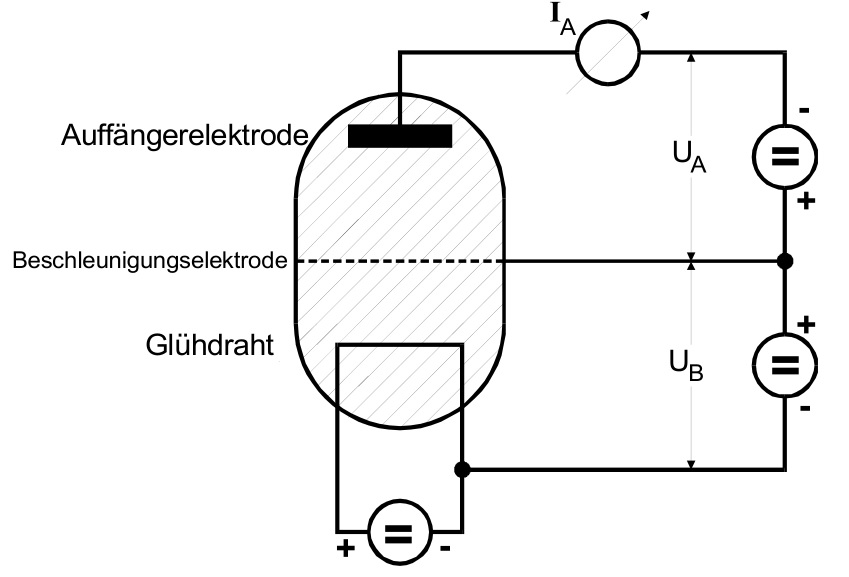
\includegraphics[height=4.0cm]{data/abb1.jpg}
    \caption{Braggsche Reflexion am Gitter. \cite{V601}}
    \label{fig:abb1}
\end{figure}
In Abb. \ref{fig:abb1} ist eine schematische Darstellung des Franck-Hertz-Versuchs zu sehen.
Im Ovalen Gefäß befindet sich Quecksilber, welches zum Teil spontan verdampft, bis sich ein Gleichgewichtsdampfdruck einstellt.
Dieser Druck $p_{Sättigung}$ hängt nur von der Temperatur ab.
Durch einen Gleichstrom wird der Glühdraht erhitzt, welcher durch den glühelektrischen Effekt Elektronen emmittiert.
Gegenüber ist eine Elektrode mit der positiven Spannung $U_B$, zu welcher die Elektronen hin beschleunigt werden.
Anschließend besitzen die Elektronen eine kinetische Energie von:
\begin{equation}
    \frac{\text{m}_0 v_{vor}^2}{2} = \text{e}_0 U_B
    \label{eqn:gl2}
\end{equation}
Diese Gleichung gilt nur, wenn die Elektronen zuvor die Geschwindigkeit v = 0 hatten.
Hinter der Beschleunigungselektrone wird eine negativ geladene Auffängerelektrode gesetzt.
Nur die Elektronen, deren Geschwindigkeit $v_z$ in Feldrichtung die Ungleichung
\begin{align*}
    \frac{\text{m}_0}{2}v_z^2 >= \text{e}_0 U_A
\end{align*}
erfüllt, kommen an der Auffängerelektrode an, die anderen kehren zur Beschleunigungselektrode zurück.
Bei nur geringer Energie der Elektronen treten lediglich elastische Stöße im Beschleunigerraum auf.
Durch das Massenverhältnis $\frac{\text{m}_0}{\text{M}}$, welches den Energieverlust bestimmt und sehr klein ist.
Ist bei den elastischen Stößen der Energieverlust $\Delta E$ des Elektrons nicht von Relevanz.
\begin{align*}
    \Delta E 0 \frac{4 \text{m}_0 \text{M}}{(\text{m}_0 + \text{M})^2} \cdot E \approx 1,1 \cdot 10^{-5} E
\end{align*}
Während der Energieverlust also zu vernachlässigen ist, muss die Richtungsänderung, die das Elektron bei dem Stoß erfährt, trotzdem beachtet werden.
Wird die Energie der Elektronen genauso groß wie die Energiedifferenz $E_1 -E_0$ oder größer, so kommt es zu unelastischen Stößen zwischen ihnen und den Hg-Atomen.
Dadurch wird das Hg-Atom mit der Energiedifferenz auf den angeregten Zustand gehoben und das Elektron behält die restliche Energie.
Das Hg-Atom geht vom ersten angeregten Zustand unter Emission einer elektromagnetischen Welle wieder in den Grundzustand über.
Das emittierte Lichtquant besitzt die Energie:
\begin{equation}
    \text{h} \nu = E_1 - E_0
    \label{eqn:gl3}
\end{equation}
\nu ist die Frequenz der emittierte Strahlung und h das Plancksche Wirkungsquantum.
Bei der Gegenfeldmethode wird nun der Strom $I_A$ an der Auffängerkathode beobachtet, wobei die Beschleunigungsspannung $U_B$ kontinuierlich vergrößert wird. 
Ein schematischer Verlauf der Kurve ist in Abbildung \ref{fig:abb2} zu sehen. 
\begin{figure}
    \centering
    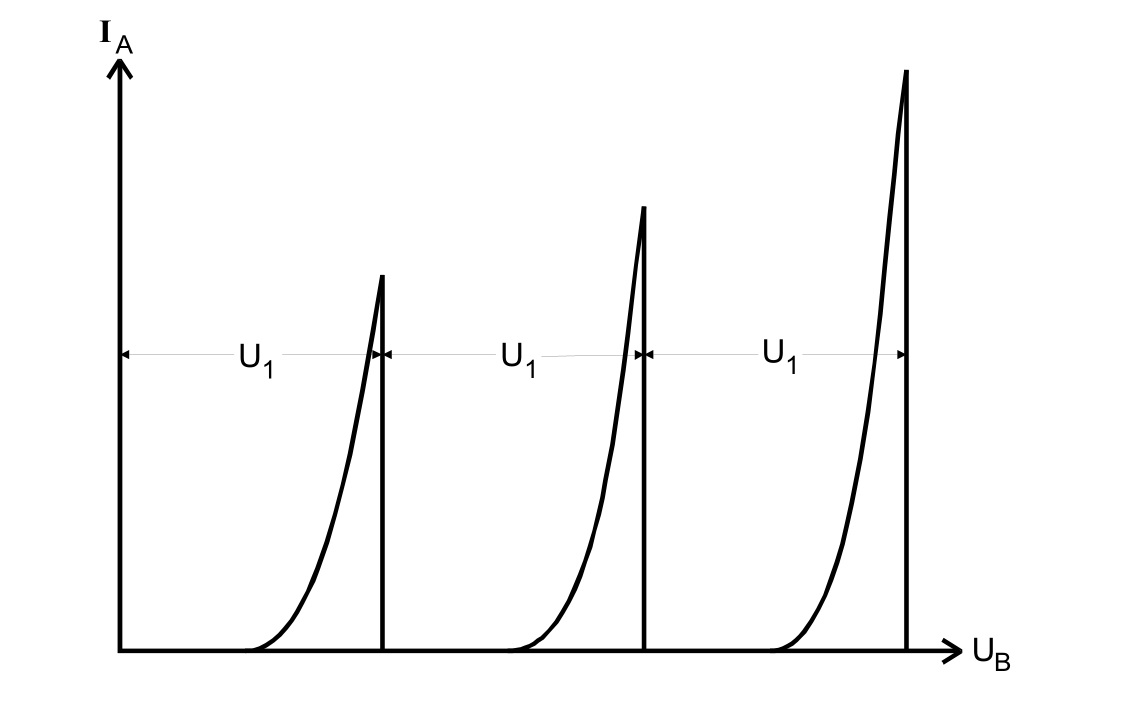
\includegraphics[height=4.0cm]{data/abb2.jpg}
    \caption{Zusammenhang zwischen $U_B$ und $I_A$.  \cite{V601}}
    \label{fig:abb2}
\end{figure}
Es wird ein größer werdender Strom registreiert, wenn die Beschleunigungsspannung größer ist als die Spannung der Auffängerelektrode.
Sobald die Elektronen die Energie von $E_1 - E_0$ erreichen verlieren sie die Energie bei den unelstischen Stößen und gelangen nicht mehr zur Auffängerkathode.
Bei weiterer Steigerung der Beschleunigungsspannung erhalten die Elektronen nach dem Stoß erneut Energie, bis sie wieder den Energiebetrag $E_1 -E_0$ besitzen und erneut ein Hg-Atom anregen können.
Der Auffängerstrom wird also in periodischen Intervallen der Länge $U_1$ immer wieder ansteigen und abrupt abfallen. 
Die Länge $U_1$ bezeichnet das erste Anregungspotential:
\begin{equation}
    U_1 := \frac{1}{\text{e}_0}(E_1 - E_0)
    \label{eqn:gl4}
\end{equation}

\subsection{Störeinflüsse}
\label{Stoer}

In einigen Punkten weicht die beobachtete Kurve des Auffängerstroms vom Idealfall ab.
Sowie das Beschleunigungspotential von der Beschleunigungsspannung abweicht.
Dies liegt an den unterschiedlichen Austrittsarbeiten für Elektronen des Glühdrahts und der Beschleunigungselektrode.
Für das effektive Beschleunigungspotential ergibt sich:
\begin{equation}
    U_{B,eff} = U_B - \frac{1}{\text{e}_0}(\Phi_B - \Phi_G)
    \label{eqn:gl5}
\end{equation}
\Phi ist die Austrittsarbeit des Glühdrahts, bzw der Beschleunigungselektrode.
$\frac{1}{\text{e}_0}(\Phi_B - \Phi_G)$ wird als Kontaktpotential K bezeichnet.
Desweiteren treten die Elektronen schon mit einer von Null verschiedenen Anfangsgeschwindigkeit aus dem Metall aus.
Deswegen besitzen sie nach dem Durchlauf eine Energieverteilung, was dazu führt, dass es nicht bei einer genau zu bestimmenden Beschleunigungsspannung zu unelastischen Stößen kommt.
Somit wird sich die Kurve den Maxima flacher annähern und stetig einem Minimum annähern.
Durch die elastischen Stöße und die daraus folgenden Richtungsänderungen kommt es zu einer Verteilung  der relevanten Geschwindigkeitskomponente $v_z$.
Dadurch erreichen nicht mehr alle Elektronen die Auffängerelektrode.